% Template for Cogsci submission with R Markdown

% Stuff changed from original Markdown PLOS Template
\documentclass[10pt, letterpaper]{article}

\usepackage{cogsci}
\usepackage{pslatex}
\usepackage{float}
\usepackage{caption}

% amsmath package, useful for mathematical formulas
\usepackage{amsmath}

% amssymb package, useful for mathematical symbols
\usepackage{amssymb}

% hyperref package, useful for hyperlinks
\usepackage{hyperref}

% graphicx package, useful for including eps and pdf graphics
% include graphics with the command \includegraphics
\usepackage{graphicx}

% Sweave(-like)
\usepackage{fancyvrb}
\DefineVerbatimEnvironment{Sinput}{Verbatim}{fontshape=sl}
\DefineVerbatimEnvironment{Soutput}{Verbatim}{}
\DefineVerbatimEnvironment{Scode}{Verbatim}{fontshape=sl}
\newenvironment{Schunk}{}{}
\DefineVerbatimEnvironment{Code}{Verbatim}{}
\DefineVerbatimEnvironment{CodeInput}{Verbatim}{fontshape=sl}
\DefineVerbatimEnvironment{CodeOutput}{Verbatim}{}
\newenvironment{CodeChunk}{}{}

% cite package, to clean up citations in the main text. Do not remove.
\usepackage{apacite}

% KM added 1/4/18 to allow control of blind submission


\usepackage{color}

% Use doublespacing - comment out for single spacing
%\usepackage{setspace}
%\doublespacing


% % Text layout
% \topmargin 0.0cm
% \oddsidemargin 0.5cm
% \evensidemargin 0.5cm
% \textwidth 16cm
% \textheight 21cm

\title{Why Verbs Are Harder to Learn Than Nouns: A Quantitative Approach}


\author{{\large \bf Morton Ann Gernsbacher (MAG@Macc.Wisc.Edu)} \\ Department of Psychology, 1202 W. Johnson Street \\ Madison, WI 53706 USA \AND {\large \bf Sharon J.~Derry (SDJ@Macc.Wisc.Edu)} \\ Department of Educational Psychology, 1025 W. Johnson Street \\ Madison, WI 53706 USA}


\begin{document}

\maketitle

\begin{abstract}
Include no author information in the initial submission, to facilitate
blind review. The abstract should be one paragraph, indented 1/8 inch on
both sides, in 9\textasciitilde point font with single spacing. The
heading `Abstract' should be 10\textasciitilde point, bold, centered,
with one line of space below it. This one-paragraph abstract section is
required only for standard six page proceedings papers. Following the
abstract should be a blank line, followed by the header `Keywords' and a
list of descriptive keywords separated by semicolons, all in
9\textasciitilde point font, as shown below.

\textbf{Keywords:}
Add your choice of indexing terms or keywords; kindly use a semi-colon;
between each term.
\end{abstract}

By the time they are two years old, children fill out their vocabularies
with hundreds of words - many of these are nouns like ``dog'' and
``ball'', but others are social performatives or proto-verbs like
``bye'' and ``up'' (Braginsky, Yurovsky, Marchman, \& Frank, 2019;
Tardiff et al., 2008).

(Behavior experiment evidence suggests that children learn a
disproportionate amount of nouns in their early age.) The core
difference is that verbs are more variable than nouns in various ways
(Gentner). First, verbs are more variable in their semantics. One verb
can be used to mention several actions, and one action can always be
described by more than one verb. Second, verb meanings are more variable
across languages, while nouns are relatively stable
cross-linguistically. Finally, verbs are more variable in terms of word
forms. More cognitive capacity is needed for children in order to figure
out that different verb forms actually correspond to the same concept of
verb.

To explain the phenomena from theory level, we examine different
learning theories.

One possibility is that children learn cross-modal mappings directly
from the co-occurrence statistics between the words they hear and their
observations of the world around them. Although the referent of a word
may be ambiguous in any individual context, children could learn a
word's meaning by identifying what is consistent across the many
contexts of its use (Siskind, 1996; Yu \& Smith, 2007). That is, a child
could learn that ``ball'' generally refers to round toys because it is
frequently used when they are around. Evidence from a number of labs now
shows that children and even infants can use cross-situational
statistical information to learn the meanings of concrete nouns in
simplified contexts (Smith \& Yu, 2008; Vlach \& Johnson, 2013; Suanda
et al., 2014).

However, there are reasons to think that children do not learn all of
these words by tracking cross-modal occurrence information. First,
referential ambiguity in the world may be significantly more complex
than the ambiguity faced by children in these lab studies (Medina et
al., 2013; although c.f. Yurovsky et al., 2012). One extreme case of
this is that words may refer not to co-present objects, but instead to
things in the past or future. As Gleitman (1990) points out, a child's
caregiver is unlikely to say `` I am opening the door!'' as they come
home from work, but instead something like ``It's freezing outside!''.
Second, studies showing successful cross-situational learning of
non-noun meanings are rare, and successes have been found only in older
children with significant extra scaffolding (Childers \& Paik, 2009;
Scott \& Fisher, 2012).

An alternative possibility is that children learn meanings not from
cross modal correspondence but from the structure of information within
individual modalities. An intriguing body of evidence consistent with
this possibility comes from the semantics of children who do not have
access to visual information. Blind children--who cannot learn the
meanings of words by mapping them onto their visual referents--have very
similar semantics for highly visual words as sighted children (Landau,
et al., 1985). Even sighted children develop an early understanding of
the category of color words before they learn the meanings of the words
themselves. That is, two-year-olds know that the right answer for a
question like ``what color is this'' is ``blue'' or ``green'' rather
than ``dog'' even if they cannot correctly identify which color is the
right answer (Bartlett, 1978). Statistical models trained on corpora of
English language are able to recover a striking amount of information
about the meanings of words, even without the complex machinery that has
enabled modern machine learning models to be so powerful (Lund \&
Burgess, 1996; Landauer \& Dumais, 1997). But how could children ground
these linguistic ``meanings'' in the physical world; how could these
uni-modal meanings be used for cross-modal mapping without tracking
cross-modal co-occurrence?

\hypertarget{alignment-theory}{%
\subsection{Alignment Theory}\label{alignment-theory}}

Recently, Roads and Love (2020) proposed a novel and interesting
learning theory, which ingeniously excludes any use of cross-modality
co-occurrence statistics - they view word learning as the unsupervised
alignment of multiple conceptual systems (e.g., visual system, language
system, acoustic system). {[}An example: dog, cat, tiger{]}. The key
insight is that different sources of input should produce similar
conceptual systems because sources are different viewpoints of the same
underlying reality. If structural idiosyncrasies present in one system
are qualitatively mirrored in the other system, then it is possible to
align the two systems. Technically, the alignment is done in two steps.
At step one, the learner infers the distribution of concepts within each
independent modality by measuring the similarity of each pair of
concepts. Once the learner has a good sense of the similarity structures
of concepts within each conceptual system, at step two, the mapping of
all concepts across systems can be set up at one go: Roads and Love
discovered that the alignment correlation of two systems positively
correlates with the mapping accuracy, which implies that the alignment
correlation can be used as a hint to find the perfect mapping {[}one
figure here{]}. {[}brief discussion: 1. Both cross-situational learning
and the alignment idea are unsupervised methods. 2. The core difference
is that in alignment theory, no cross-modality co-occurrence statistics
is needed.{]} We use this alignment idea as an alternate framework to
explore the verb problems from before

For more information on citations in RMarkdown, see
\textbf{\href{http://rmarkdown.rstudio.com/authoring_bibliographies_and_citations.html\#citations}{here}.}

\hypertarget{study-0}{%
\section{Study 0}\label{study-0}}

As we mentioned before, one of Roads and Love's most important findings
is that the alignment correlations of systems positively correlate with
the mapping accuracy of concepts, which suggests that better mapping
usually co-occurs with higher alignment correlation.

We first verify this finding by replicating Roads and Love's experiment
of noun concept alignment on a new dataset, using new embedding models.
We demonstrated the alignment across the visual system and the language
system.

\hypertarget{footnotes}{%
\subsection{Footnotes}\label{footnotes}}

Indicate footnotes with a number\footnote{Sample of the first
footnote.} in the text. Place the footnotes in 9 point type at the
bottom of the page on which they appear. Precede the footnote with a
horizontal rule.\footnote{Sample of the second footnote.} You can also
use markdown formatting to include footnotes using this
syntax.\footnote{Sample of a markdown footnote.}

\hypertarget{figures}{%
\subsection{Figures}\label{figures}}

All artwork must be very dark for purposes of reproduction and should
not be hand drawn. Number figures sequentially, placing the figure
number and caption, in 10 point, after the figure with one line space
above the caption and one line space below it. If necessary, leave extra
white space at the bottom of the page to avoid splitting the figure and
figure caption. You may float figures to the top or bottom of a column,
or set wide figures across both columns.

\hypertarget{two-column-images}{%
\subsection{Two-column images}\label{two-column-images}}

You can read local images using png package for example and plot it like
a regular plot using grid.raster from the grid package. With this method
you have full control of the size of your image. \textbf{Note: Image
must be in .png file format for the readPNG function to work.}

You might want to display a wide figure across both columns. To do this,
you change the \texttt{fig.env} chunk option to \texttt{figure*}. To
align the image in the center of the page, set \texttt{fig.align} option
to \texttt{center}. To format the width of your caption text, you set
the \texttt{num.cols.cap} option to \texttt{2}.

\begin{CodeChunk}
\begin{figure*}[h]

{\centering 
\includegraphics{figs/2-col-image-1} 

}

\caption[This image spans both columns]{This image spans both columns. And the caption text is limited to 0.8 of the width of the document.}\label{fig:2-col-image}
\end{figure*}
\end{CodeChunk}

\hypertarget{one-column-images}{%
\subsection{One-column images}\label{one-column-images}}

Single column is the default option, but if you want set it explicitly,
set \texttt{fig.env} to \texttt{figure}. Notice that the
\texttt{num.cols} option for the caption width is set to \texttt{1}.

\begin{CodeChunk}
\begin{figure}[H]

{\centering 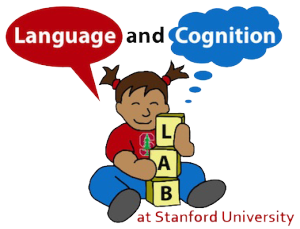
\includegraphics{figs/image-1} 

}

\caption[One column image]{One column image.}\label{fig:image}
\end{figure}
\end{CodeChunk}

\hypertarget{r-plots}{%
\subsection{R Plots}\label{r-plots}}

You can use R chunks directly to plot graphs. And you can use latex
floats in the fig.pos chunk option to have more control over the
location of your plot on the page. For more information on latex
placement specifiers see
\textbf{\href{https://en.wikibooks.org/wiki/LaTeX/Floats,_Figures_and_Captions}{here}}

\begin{CodeChunk}
\begin{figure}[H]

{\centering 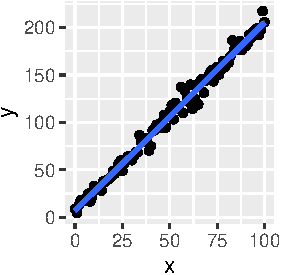
\includegraphics{figs/plot-1} 

}

\caption[R plot]{R plot}\label{fig:plot}
\end{figure}
\end{CodeChunk}

\hypertarget{tables}{%
\subsection{Tables}\label{tables}}

Number tables consecutively; place the table number and title (in 10
point) above the table with one line space above the caption and one
line space below it, as in Table 1. You may float tables to the top or
bottom of a column, set wide tables across both columns.

You can use the xtable function in the xtable package.

\begin{table}[H]
\centering
\begin{tabular}{rrrrr}
  \hline
 & Estimate & Std. Error & t value & Pr($>$$|$t$|$) \\ 
  \hline
(Intercept) & 0.03 & 0.10 & 0.3 & 0.74 \\ 
  x & 2.02 & 0.10 & 21.1 & 0.00 \\ 
   \hline
\end{tabular}
\caption{This table prints across one column.} 
\end{table}

\hypertarget{acknowledgements}{%
\section{Acknowledgements}\label{acknowledgements}}

Place acknowledgments (including funding information) in a section at
the end of the paper.

\hypertarget{references}{%
\section{References}\label{references}}

\setlength{\parindent}{-0.1in} 
\setlength{\leftskip}{0.125in}

\noindent

\hypertarget{refs}{}
\leavevmode\hypertarget{ref-braginsky2019}{}%
Braginsky, M., Yurovsky, D., Marchman, V. A., \& Frank, M. C. (2019).
Consistency and variability in children's word learning across
languages. \emph{Open Mind}, \emph{3}, 52--67.

\leavevmode\hypertarget{ref-gleitman1990}{}%
Gleitman, L. (1990). The structural sources of verb meanings.
\emph{Language Acquisition}, \emph{1}(1), 3--55.

\leavevmode\hypertarget{ref-siskind1996}{}%
Siskind, J. M. (1996). A computational study of cross-situational
techniques for learning word-to-meaning mappings. \emph{Cognition},
\emph{61}(1-2), 39--91.

\leavevmode\hypertarget{ref-tardiff2008}{}%
Tardiff, T., Fletcher, P., Liang, W., Zhang, Z., Kaciroti, N., \&
Marchman, V. (2008). Baby's first ten words. \emph{Development
Psychology}, \emph{44}(4), 929--938.

\leavevmode\hypertarget{ref-yu2007}{}%
Yu, C., \& Smith, L. B. (2007). Rapid word learning under uncertainty
via cross-situational statistics. \emph{Psychological Science},
\emph{18}(5), 414--420.

\bibliographystyle{apacite}


\end{document}
